\section{РЕЗУЛЬТАТЫ ВИЗУАЛИЗАЦИИ}
\label{sec:visualization}


Для большей наглядности были решено визуализировать только те жанры, которые лучше всего выделяются всеми алгоритмами классификации. Из 10 жанров были выбраны следующие:
\begin{itemize}
\item классическая музыка;
\item музыка в жанре металл;
\item музыка в жанре поп.
\end{itemize}

Визуализация проводилась над фрагментами музыкального произведения.

\subsection{Метод главных компонент} 
\label{sub:pca}
Метод главных компонент -- один из основных способов уменьшить размерность данных, потеряв наименьшее количество информации. Применяется во многих областях, таких как распознавание образов, компьютерное зрение, сжатие данных и т. п. Вычисление главных компонент сводится к вычислению собственных векторов и собственных значений ковариационной матрицы исходных данных или к сингулярному разложению матрицы данных. 



По двумерному отображению данных видно, что кластеры ярко выражены и линейно разделимы. Особой компактностью отличается музыка в жанре поп. Кластеры с классической музыкой и с музыкой в жанре металл, также ярко выражены.
\begin{figure}[h]
\centering
  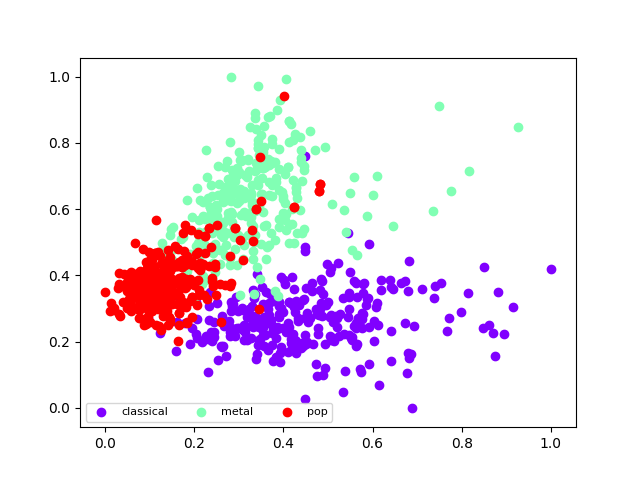
\includegraphics{2dpca.png}
  \caption{Отображения пространства  признаков музыкальных треков в двухмерное простарнство алгоритмом PCA.}
  \label{fig:results:2dtsne}
\end{figure}

Трёхмерное отображение показывает те же результаты, что и двумерная. В обоих проекциях виден малый зазор между классами.

\begin{figure}[!h]
\centering
  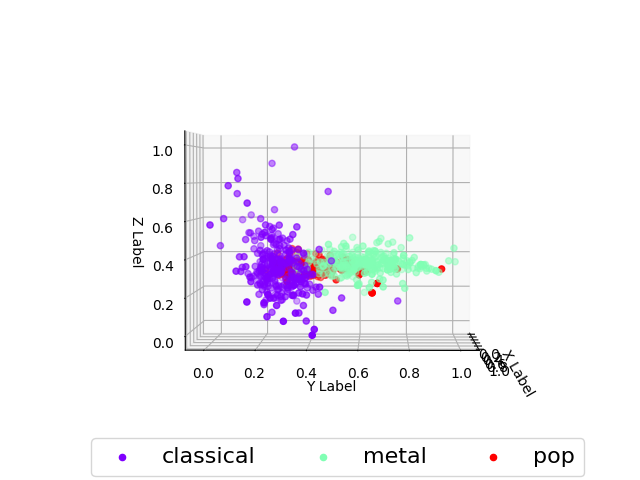
\includegraphics[scale=0.8]{3dpca1.png}
  \caption{Отображения пространства  признаков музыкальных треков в трёхмерное пространство алгоритмом PCA. Первая проекция. }
  \label{fig:results:2dtsne}
\end{figure}


\begin{figure}[!h]
\centering
  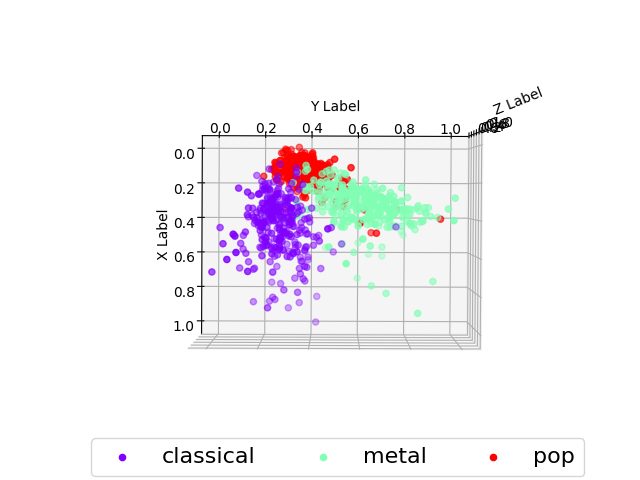
\includegraphics[scale=0.8]{3dpca2.png}
  \caption{Отображения пространства  признаков музыкальных треков в трёхмерное пространство алгоритмом PCA. Вторая проекция. }
  \label{fig:results:2dtsne}
\end{figure}


\subsection{t-SNE} 
\label{sub:tsne}
t-SNE (t-distributed stochastic neighbor embedding, стохастическое вложение соседей с распределением Стьюдента) -- алгоритм уменьшения размерности.

Точка данных (data point) – это точка $ x_i $ в исходном пространстве данных $ R^D $ (data space), где $  D $ – размерность (dimensionality) пространства данных.

Точка отображения (map point) – это точка $ y_i $ в пространстве отображения $ R^2 $ (map space). Это пространство будет содержать целевое представление набора данных.

 Более конкретно, если две точки данных расположены близко друг к другу, необходилм, чтобы две соответствующие точки отображения также располагались близко друг к другу. Пусть $  \vert x_i -  x_j \vert $ – евклидово расстояние между двумя точками данных, а  $ \vert y_i - y_j \vert$ – расстояние между точками отображения. Сначала определим условное сходство (conditional similarity) для двух точек данных:
\begin{equation}\label{eq:conditionsimilarity}
p_{j \vert i}  = \frac{ exp(\frac{- \vert x_i - x_j \vert^2}{2\sigma_i^2})}{  \sum \limits_{k \neq i}^{} exp(\frac{- \vert x_i - x_j \vert^2}{2\sigma_i^2})}
\end{equation}  \\
Это выражение показывает, насколько точка $x_j$ близка к $x_i$, при гауссовом распределении вокруг $ x_i $ с заданной дисперсией $ \sigma_i^2 $. Дисперсия различна для каждой точки. Она выбирается таким образом, чтобы точки, расположенные в областях с большой плотностью, имели меньшую дисперсию, чем точки, расположенные в областях с малой плотностью. 

Теперь определим сходство, как симметричный вариант условного сходства:
\begin{equation}\label{eq:similarity}
 p_{ij} = \frac{p_{j \vert i} +  p_{i \vert j} }{2N}
\end{equation}  \\

Получаем матрицу сходства (similarity matrix) для исходного набора данных.

Также получаем матрицу сходства для точек отображения.

\begin{equation}\label{eq:qconditionsimilarity}
q_{j \vert i}  = \frac{f( \vert x_i - x_j \vert)}{  \sum \limits_{k \neq i}^{} f( \vert x_i - x_j \vert)}  
\end{equation}  \\

\begin{equation}\label{eq:f}
f(z)  = \frac{1}{  1 + z^2}  
\end{equation}  \\


Для меры сходства используется расстояния Кульбака-Лейблера между двумя распределениями ($ p_{ij} $) и ($q_{ij} $):
\begin{equation}\label{eq:distance}
KL(P \vert \vert Q) = \sum_{i,j} p_{ij} log_{q_{ij}}^{p_{ij}}
\end{equation}  \\

Данная формула выражает расстояние между двумя матрицами сходства.

Чтобы минимизировать эту величину, применим градиентный спуск. Градиент может быть вычислен аналитически:
\begin{equation}\label{eq:gradient}
\frac{ \partial KL(P \vert \vert Q)}{\partial y_i} =  4 \sum_j(p_{ij} - q_{ij})g(\vert x_i - x_j \vert)u_{ij} 
\end{equation}  \\

Здесь $ u_{ij} $ – единичный вектор, идущий от $y_j $ к $ y_i $. Этот градиент выражает сумму всех сил, приложенных к точке отображения $ i$.
\begin{equation}\label{eq:f}
g(z)  = \frac{1}{  1 + z^2}  
\end{equation}  \\

Теперь объясним, почему для точек отображения было выбрано распределение Стьюдента, в то время как для точек данных применяется нормальное распределение. Известно, что объем N-мерного шара радиуса $ r $ пропорционален $ r^N $. При больших N, если выбирать случайные точки в шаре, большинство точек будет располагаться около поверхности, и очень небольшое количество – около центра.

При уменьшении размерности набора данных, если использовать гауссово распределение для точек данных и точек отображения, мы получим дисбаланс в распределении расстояний для соседей точек. Это объясняется тем, что распределение расстояний существенно отличается для пространства большой размерности и для пространства малой размерности. Тем не менее, алгоритм пытается воспроизвести одинаковые расстояния в обоих пространствах. Этот дисбаланс создает избыток сил притяжения, что иногда приводит к неудачному отображению.

Алгоритм t-SNE решает эту проблему, используя распределение Стьюдента с одной степенью свободы (или распределение Коши) для точек отображения. В отличие от гауссова распределения, это распределение имеет значительно более «тяжелый» хвост, что позволяет компенсировать дисбаланс. Для данного сходства между двумя точками данных, две соответствующие точки отображения должны находиться намного дальше друг от друга, чтобы их сходство соответствовало сходству точек данных. Это можно увидеть на следующем графике.

Использование этого распределения обеспечивает более эффективную визуализацию данных, при которой группы точек более отчетливо отделены друг от друга.

Алгоритм t-SNE обеспечивает эффективный метод визуализации сложных наборов данных. Он успешно обнаруживает скрытые структуры в данных, демонстрирует группы и компенсирует нелинейные отклонения по измерениям.

\begin{figure}[!h]
\centering
  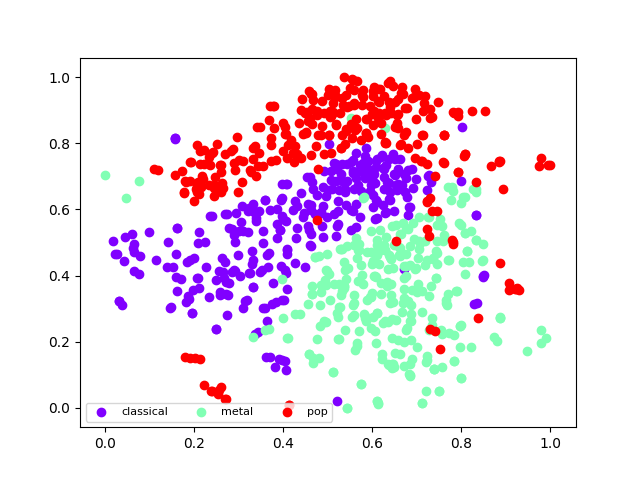
\includegraphics{vis1.png}
  \caption{Отображения пространства  признаков музыкальных треков в двухмерное простарнство алгоритмом t-SNE.}
  \label{fig:results:2dtsne}
\end{figure}

\begin{figure}[!h]
\centering
  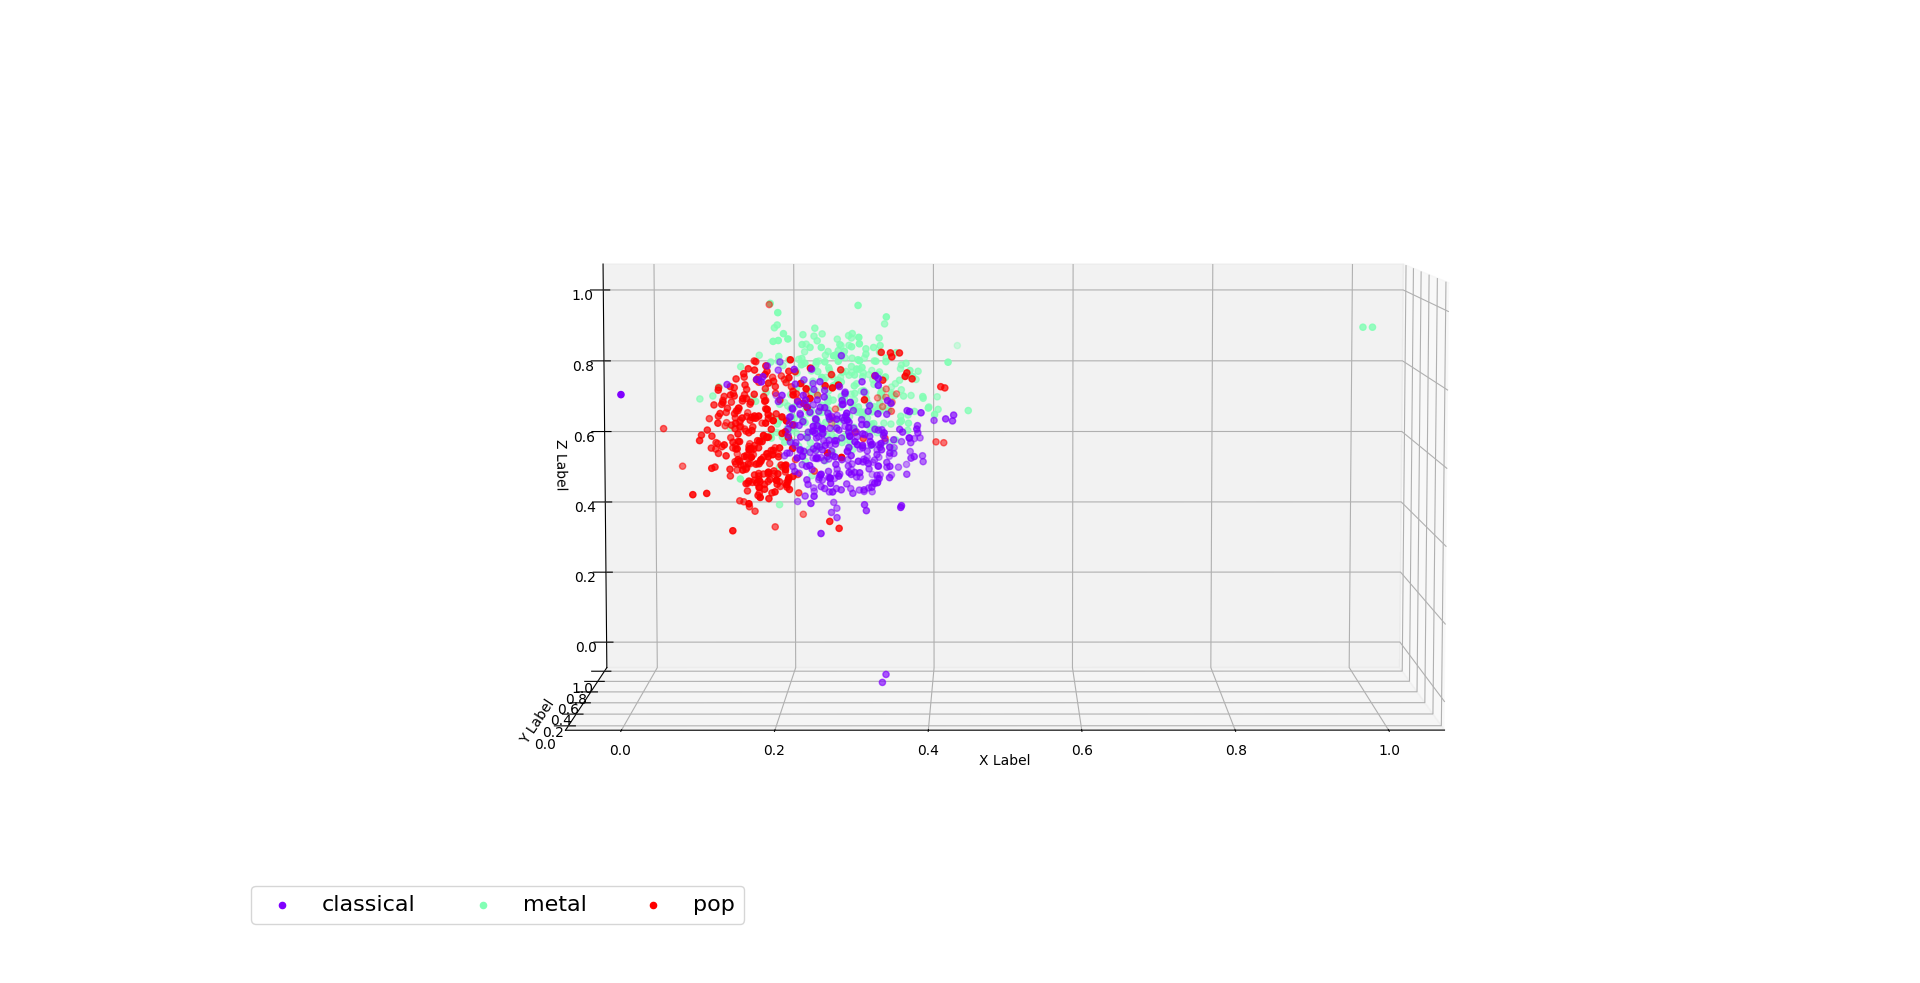
\includegraphics[scale=0.4]{3dtsne1.png}
  \caption{Отображения пространства  признаков музыкальных треков в трёхмерное пространство алгоритмом t-SNE. Первая проекция. }
  \label{fig:results:2dtsne}
\end{figure}


\begin{figure}[!h]
\centering
  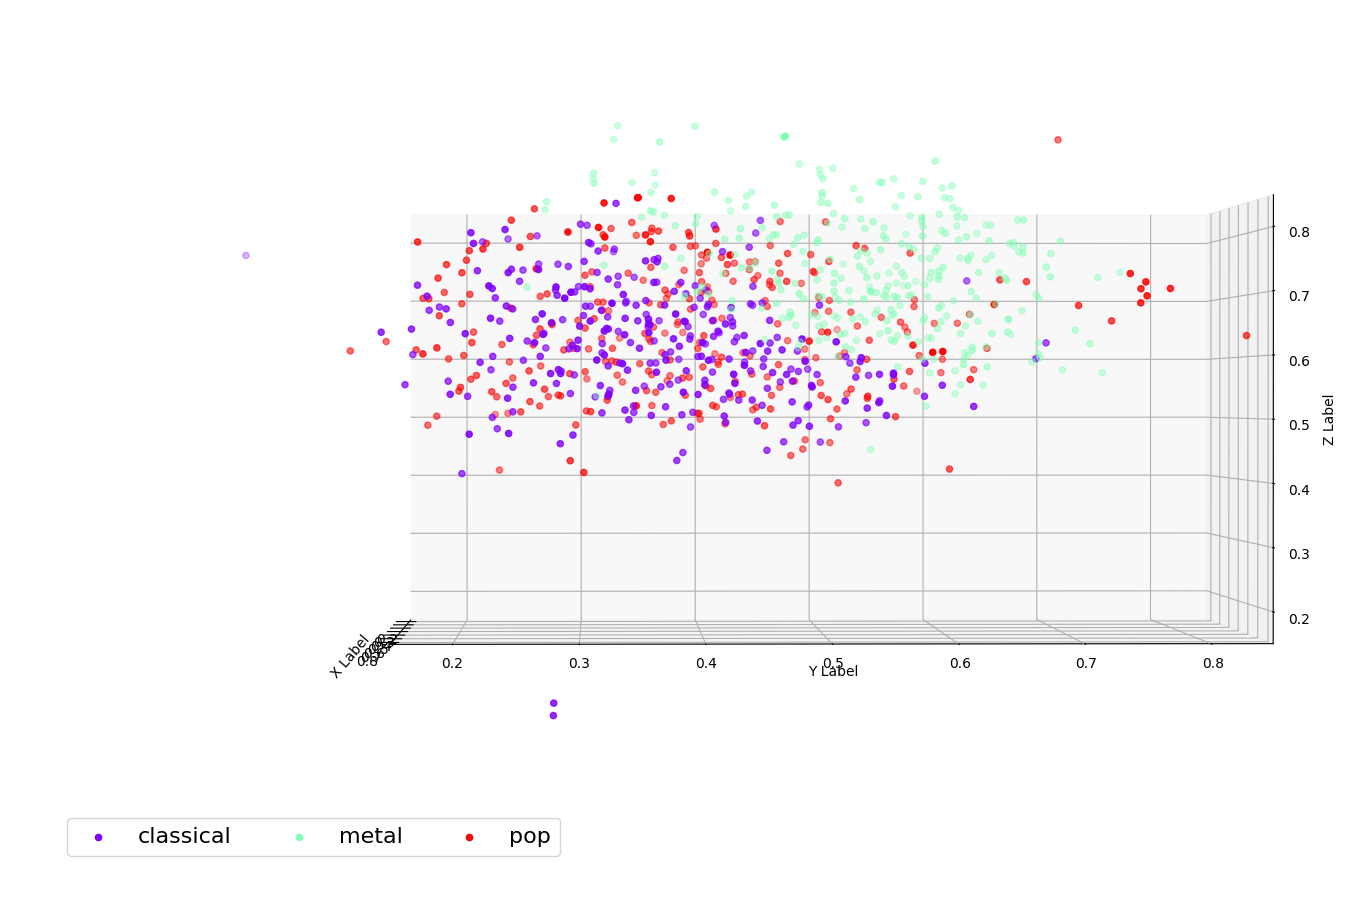
\includegraphics[scale=0.4]{3dtsne2.png}
  \caption{Отображения пространства  признаков музыкальных треков в трёхмерное пространство алгоритмом t-SNE. Вторая проекция. }
  \label{fig:results:2dtsne}
\end{figure}

Визуализация также показала, что выделенные информационные образы значимы и на их основе можно делать рекомендательный сервис. 